\chapter{Déroulement}
\section{Préparation}
Après avoir trouvé l'idée générale, nous avons commencé à esquisser quelques concept pour l'hôtel et l'ascenseur.
Pour la structure de l'hôtel, nous avions d'abord pensé à la faire entièrement en legos mais cela n'aurait pas été réalisable.
On a ensuite pensé à des profilés en aluminium mais ce n'était pas dans notre budget.
Nous avons donc décidé de découper l'hôtel dans du bois.

Nous avons d'abord modélisé grossièrement la structure sur Blender\footnote{\url{https://www.blender.org/}}, puis dessiné sur Inkscape\footnote{\url{https://inkscape.org/}} les fichiers de découpe.
Nous sommes ensuite allés aux FabLab de Sion\footnote{\url{https://fablabsion.ch/}} pour utiliser la découpeuse laser et créer un prototype du premier module, que l'on peut voir sur la figure \ref{fig:bp_prototype}.

\begin{figure}[H]
  \centering
  \raisebox{-0.5\height}{\includegraphics[width=0.6\linewidth]{building_process/thymotel_laser}}
  \raisebox{-0.5\height}{\includegraphics[width=0.3\linewidth]{building_process/thymotel_laser_ecran}}
  \caption{Découpe au laser}
  \label{fig:bp_laser}
\end{figure}

\begin{figure}[H]
  \centering
  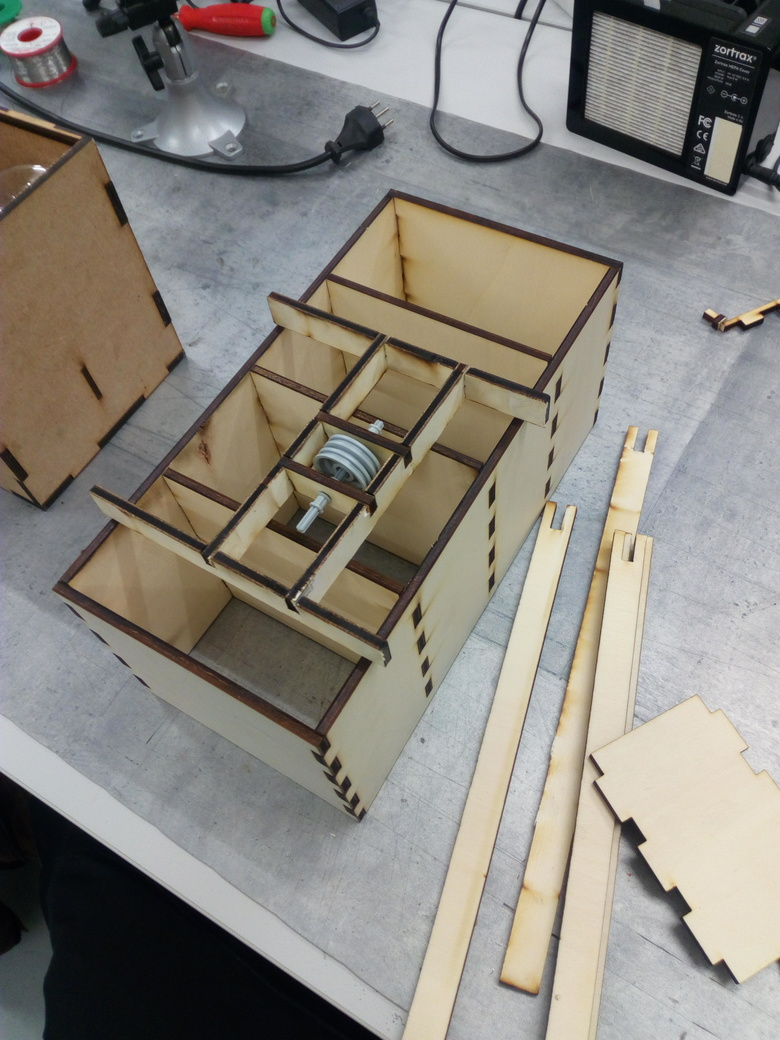
\includegraphics[scale=0.3]{building_process/prototype_module}
  \caption{Prototype d'un module}
  \label{fig:bp_prototype}
\end{figure}

Quant à l'ascenseur, nous avons imaginé de nombreuses possibilités.
Nous avions par exemple pensé à le poser sur des rails, à le tirer par en-bas ou même à le suspendre par des cables. Voici quelques croquis des différentes itérations du design de l'ascenseur.

\begin{figure}[H]
  \centering
  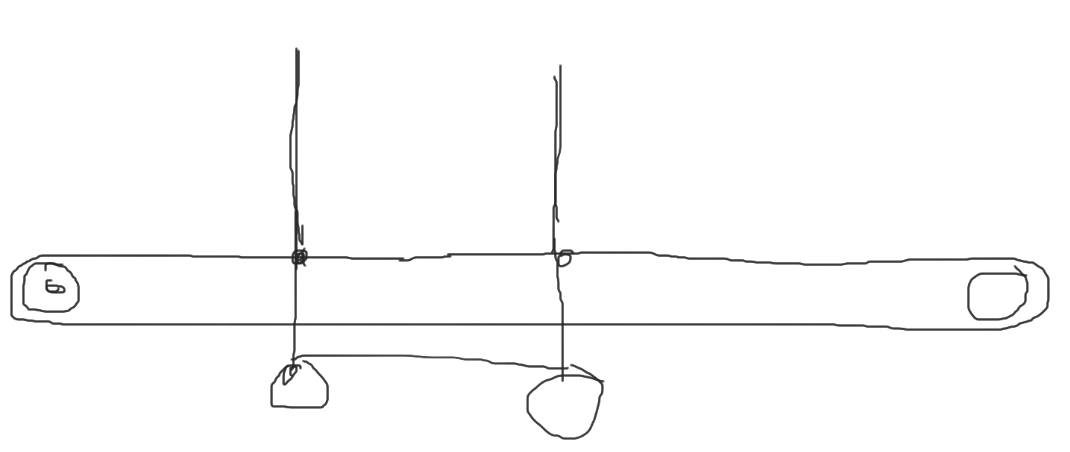
\includegraphics[width=0.4\textwidth]{croquis/boucle}
  \hspace{2em}
  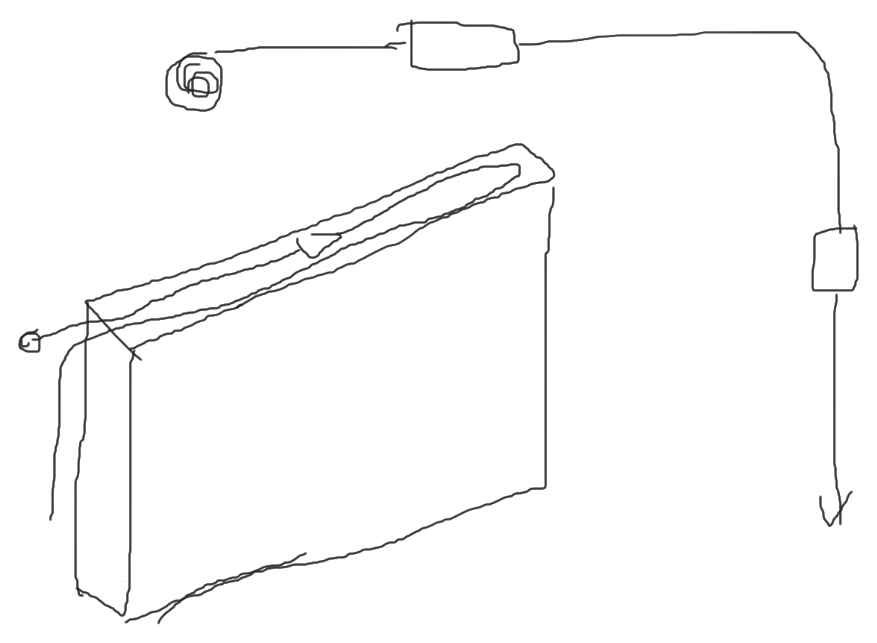
\includegraphics[width=0.4\textwidth]{croquis/boucle_dessus}
  \vspace{2em}
  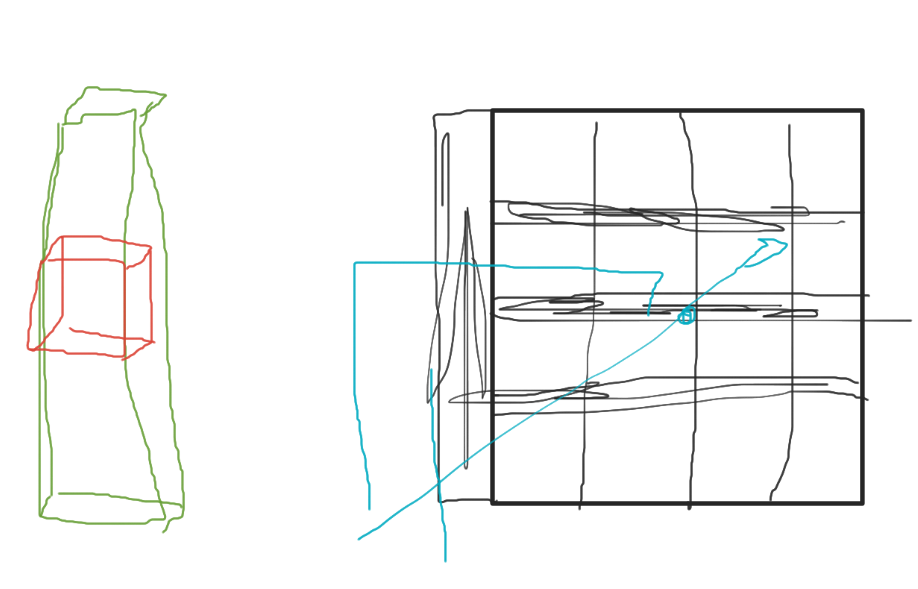
\includegraphics[width=0.4\textwidth]{croquis/hotel}
  \hspace{2em}
  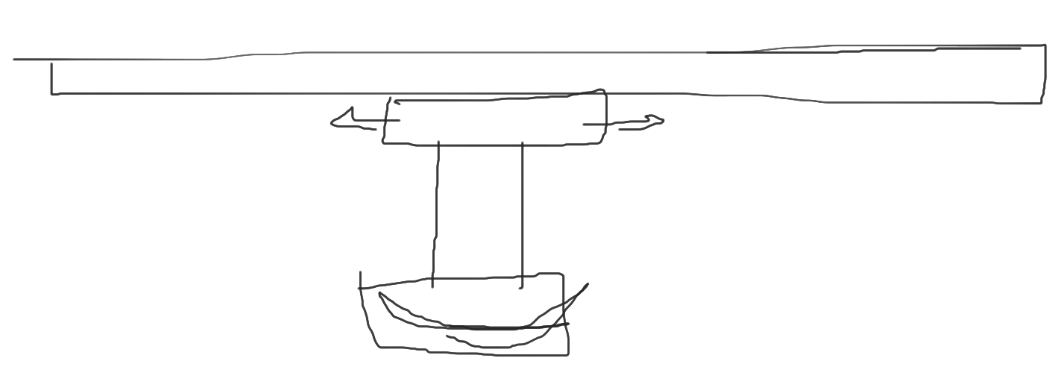
\includegraphics[width=0.4\textwidth]{croquis/palan}
  \vspace{2em}
  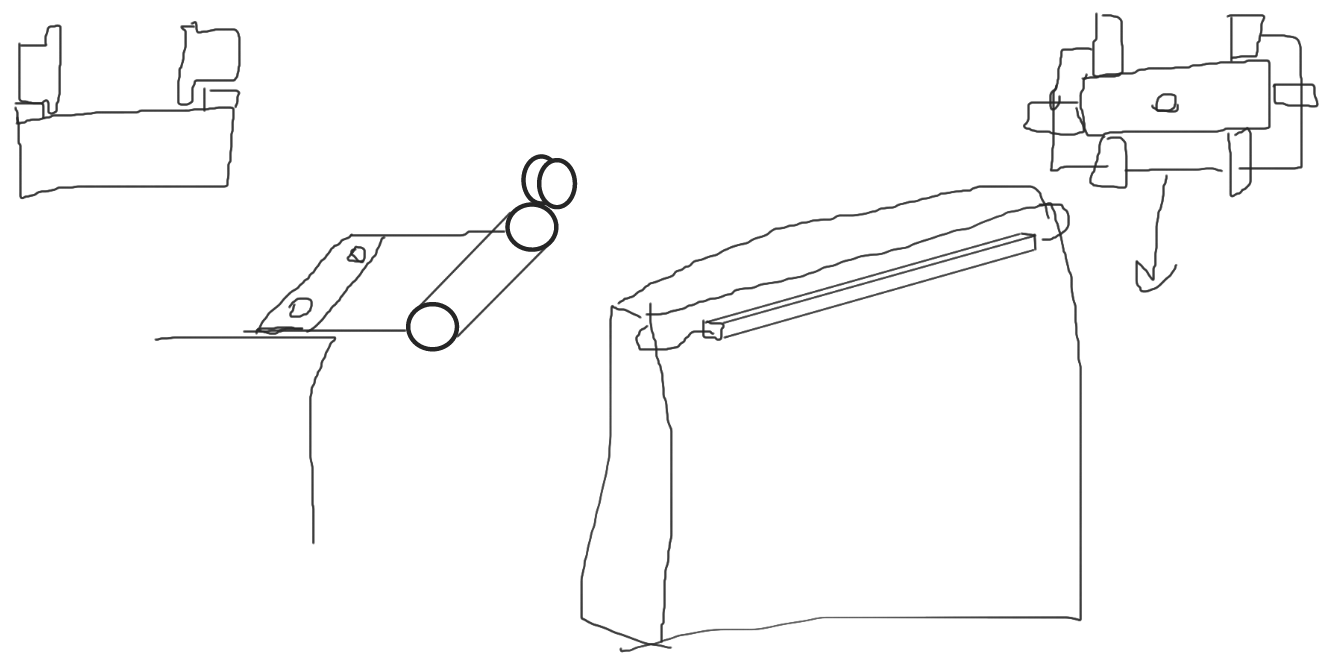
\includegraphics[width=0.4\textwidth]{croquis/roller_coaster}
  \hspace{2em}
  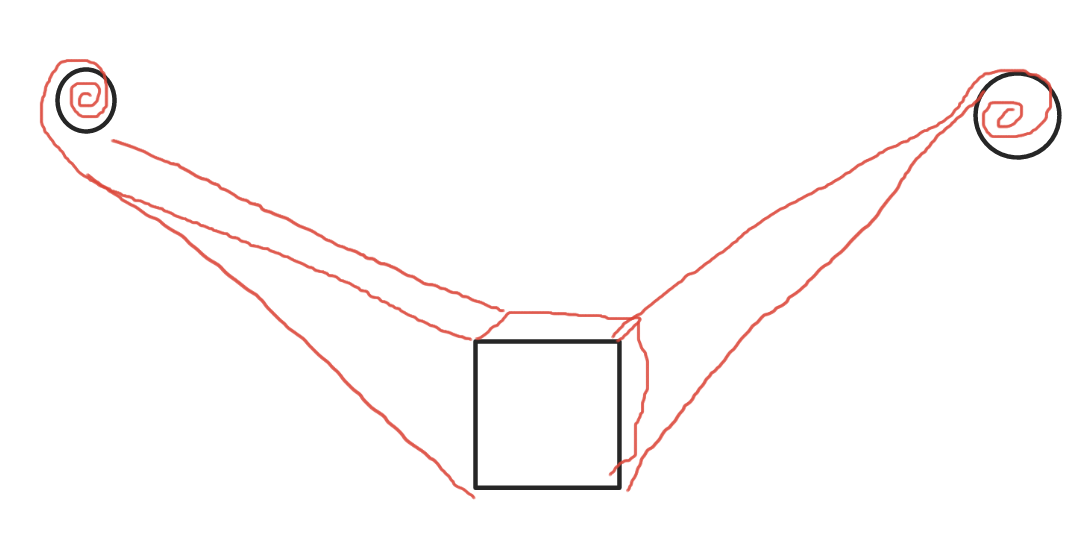
\includegraphics[width=0.4\textwidth]{croquis/suspension}
  \caption{Croquis de brainstorming}
  \label{fig:croquis}
\end{figure}

Nous avons finalement opté pour une tour montée sur roue, tirée par le haut, dans laquelle se déplace verticalement une cabine.

\begin{figure}[H]
  \centering
  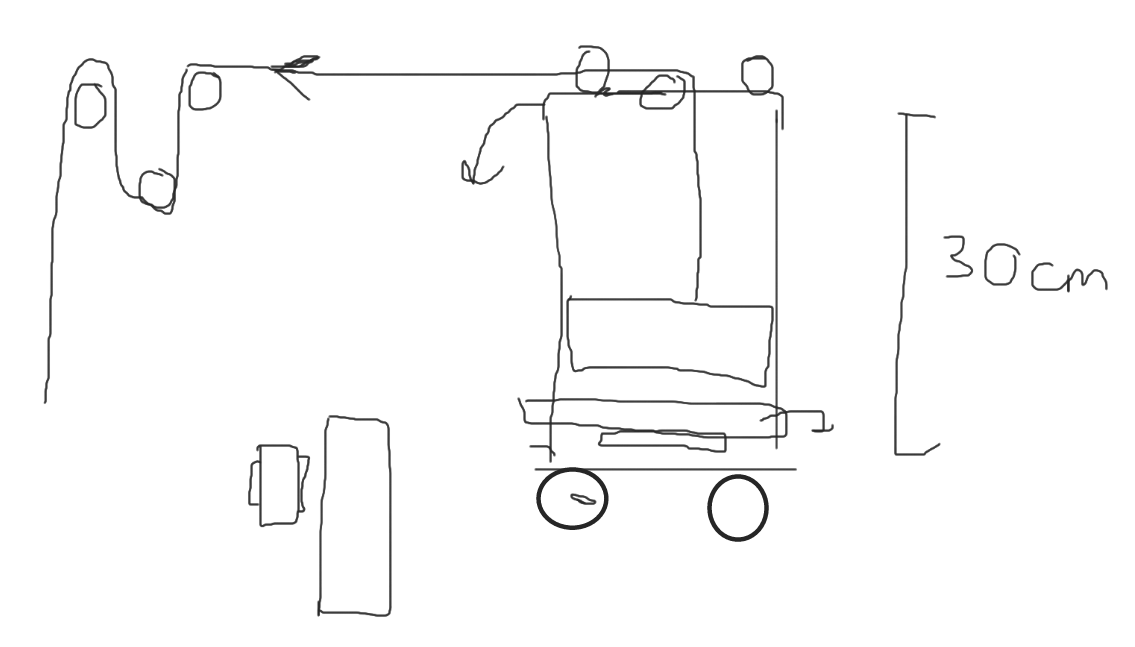
\includegraphics[width=0.8\textwidth]{croquis/contrepoid}
  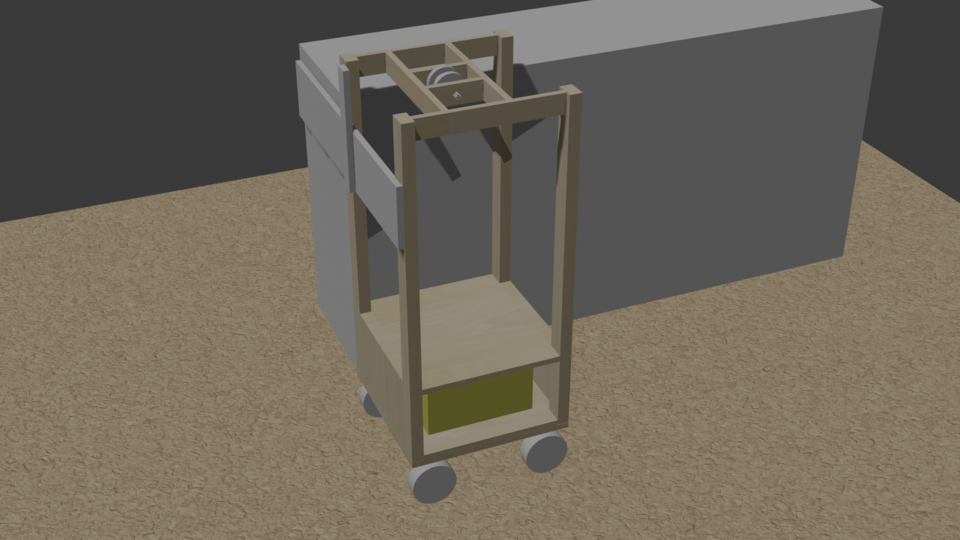
\includegraphics[width=0.8\textwidth]{croquis/ascenseur_3d}
  \caption{Modèle ascenseur}
  \label{fig:ascenseur_3d}
\end{figure}

Comme on le voit sur le croquis de la figure \ref{fig:ascenseur_3d}, la hauteur importante de la tour et les forces en jeu auraient fait basculer la structure.
Afin de résoudre ce problème et pour permettre à l'ascenseur de se déplacer vers la droite, nous avons dû installer un contrepoid tirant dans le sens opposé aux deux autres ficelles.

Du point de vue de la programmation, nous avons aussi préparé le terrain en établissant des organigrammes pour représenter l'enchaînement des étapes et des états, comme celui de l'annexe \ref{app:communication}.

Nous avons aussi défini le protocole de communication (annexe \ref{app:protocol}).

\section{Réalisation}
Après avoir découpé les différents éléments en bois, nous les avons assemblés et collés.

\begin{figure}[H]
  \centering
  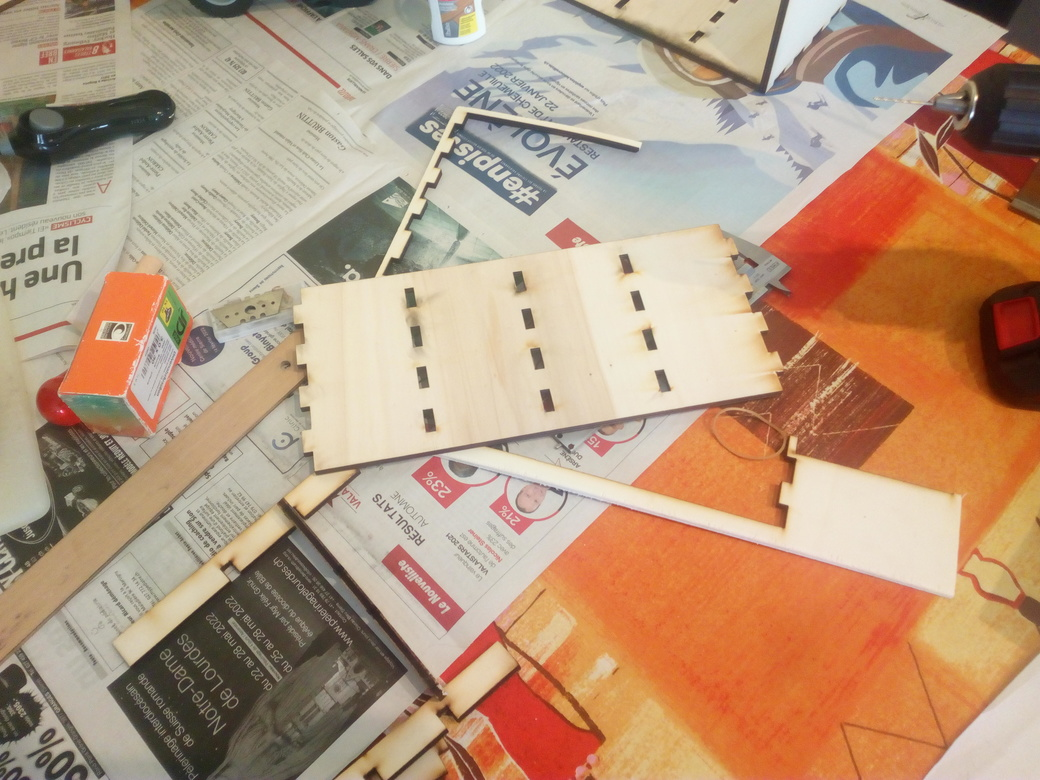
\includegraphics[width=0.4\textwidth]{building_process/assemblage_1}
  \hspace{1em}
  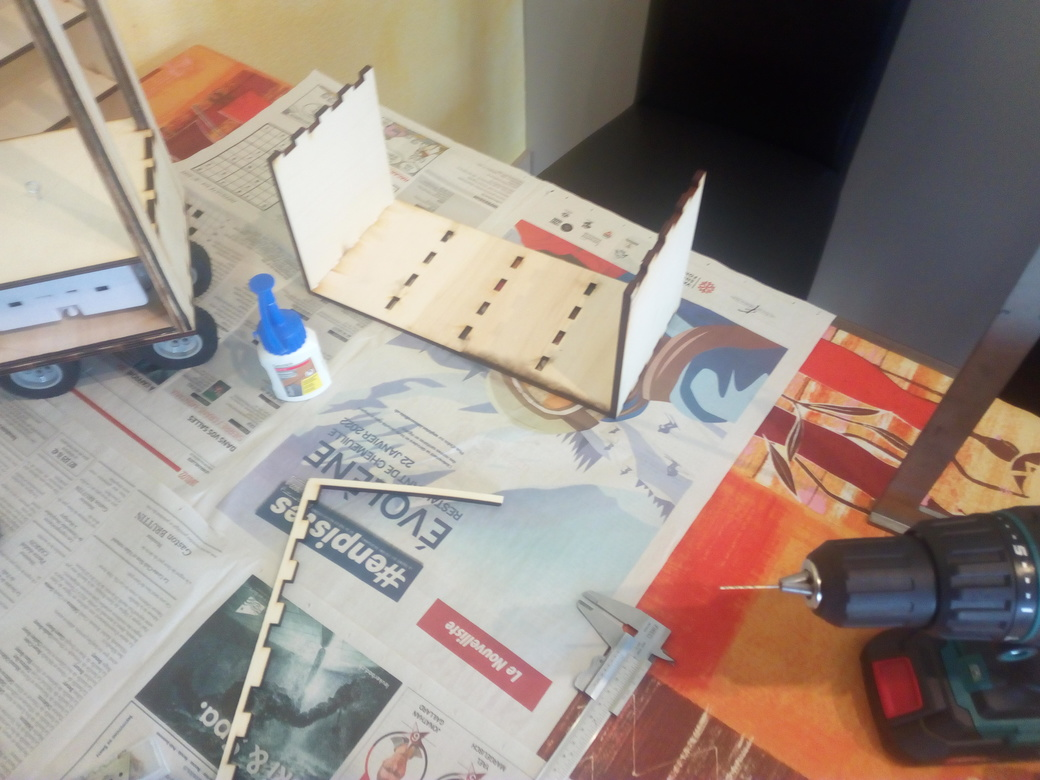
\includegraphics[width=0.4\textwidth]{building_process/assemblage_2}\\
  \vspace{1em}
  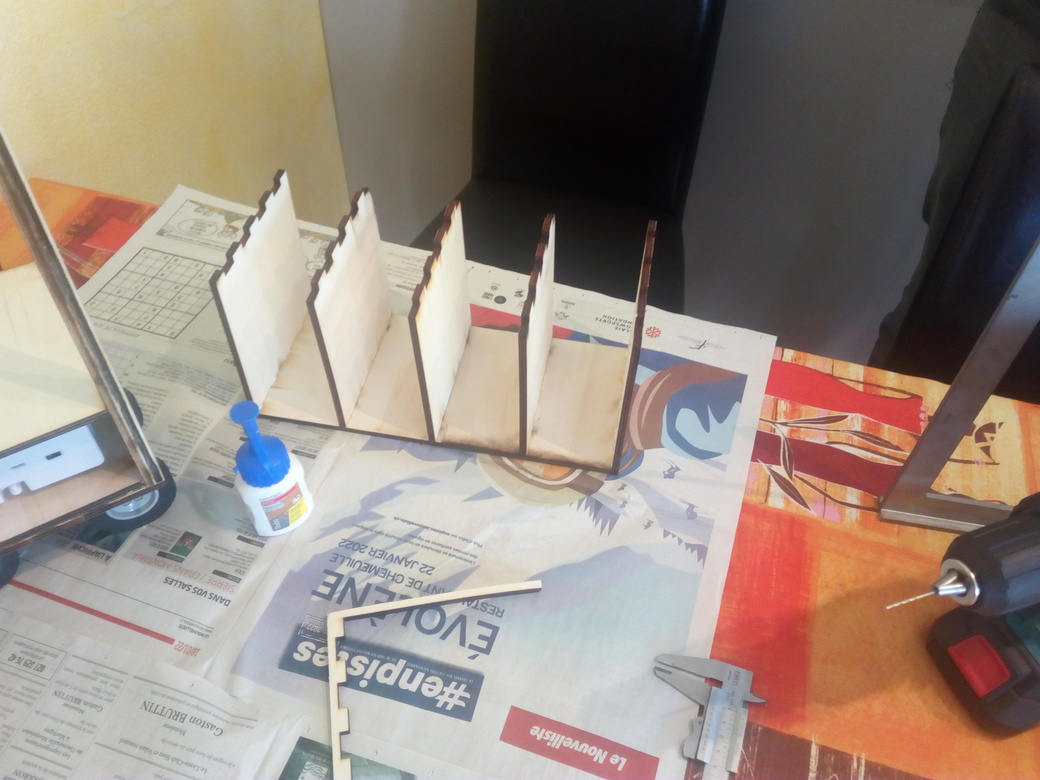
\includegraphics[width=0.4\textwidth]{building_process/assemblage_3}
  \hspace{1em}
  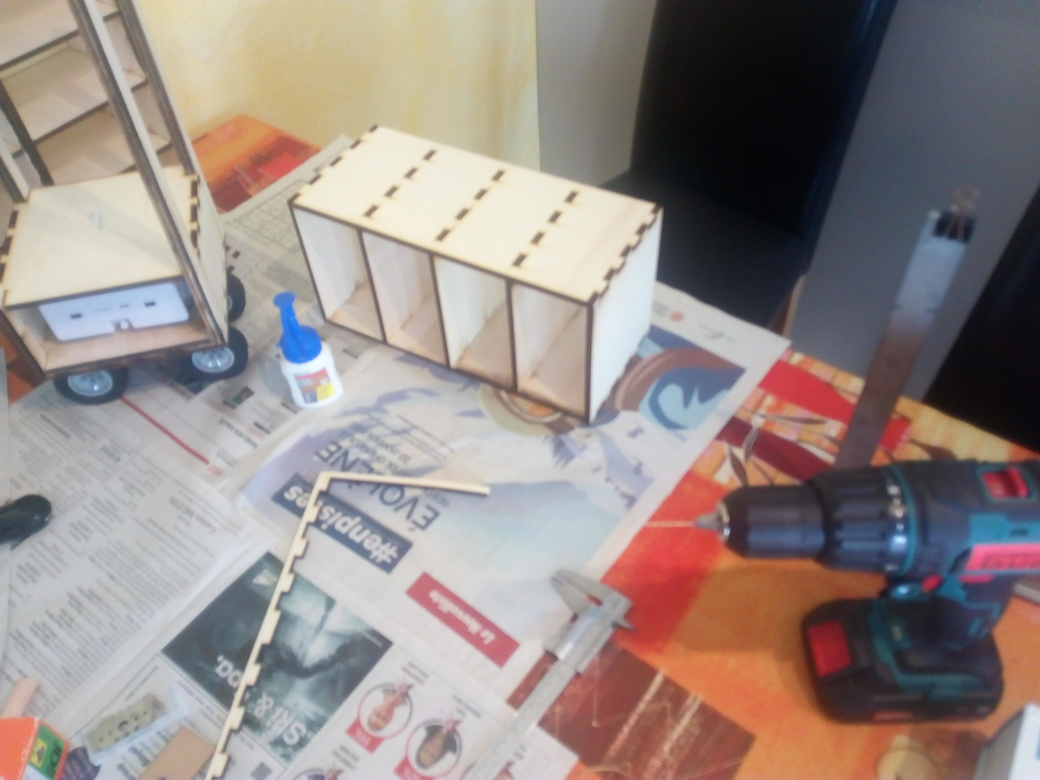
\includegraphics[width=0.4\textwidth]{building_process/assemblage_4}\\
  \vspace{1em}
  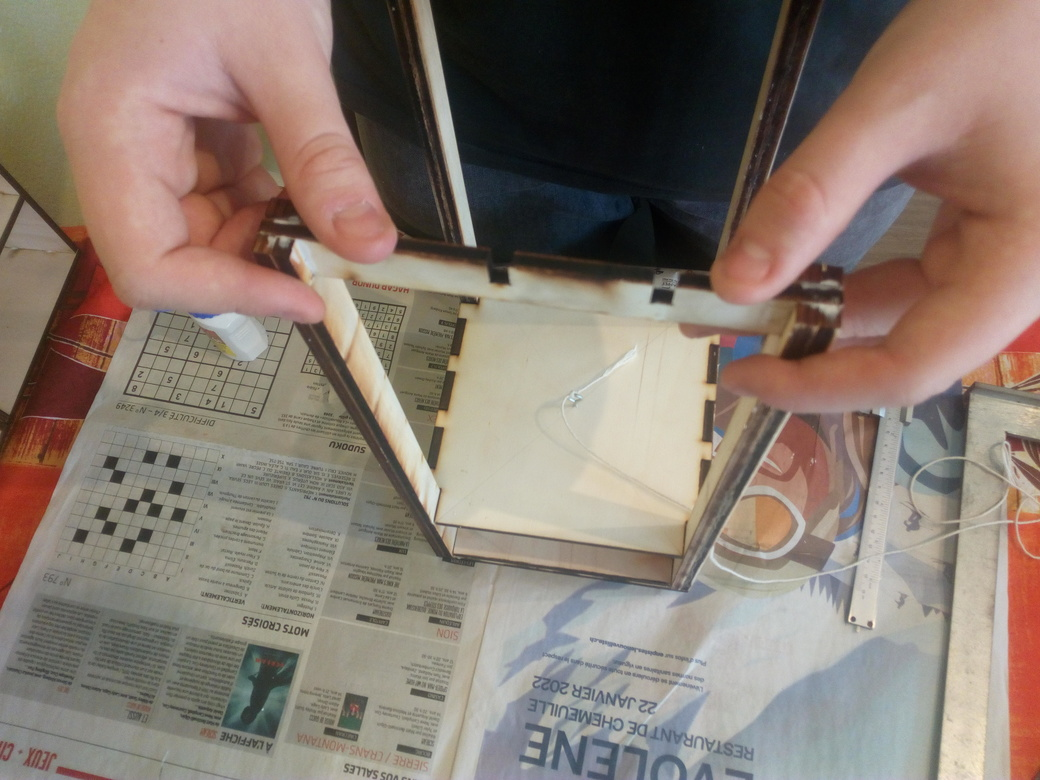
\includegraphics[width=0.4\textwidth]{building_process/assemblage_5}
  \hspace{1em}
  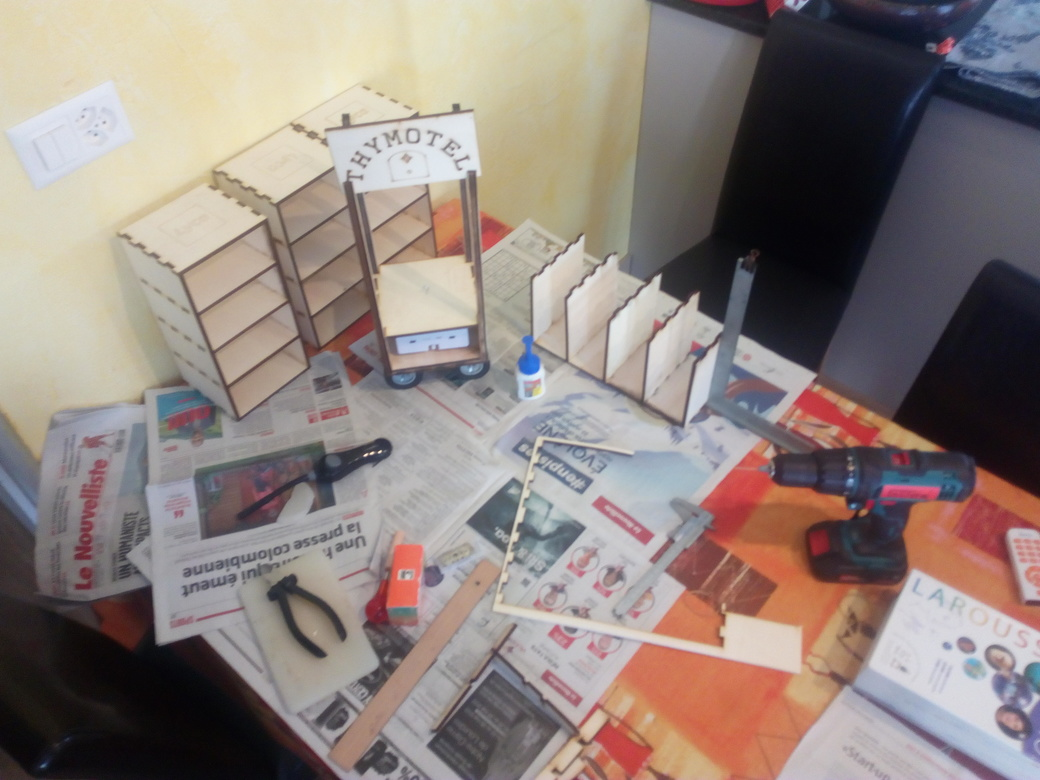
\includegraphics[width=0.4\textwidth]{building_process/assemblage_6}\\
  \caption{Assemblage}
  \label{fig:assemblage}
\end{figure}

L'assemblage ne nous a pas causé trop de problème car nous avions tout prévu à l'avance. Malheureusement, nous avons fait face à une petite difficulté.
Les tiges de soutient de la cage d'ascenseur avaient une surface de contact avec la base qui était trop petite pour que la colle les tiennent.
Nous avons donc dû les visser pour que la structure résiste aux tensions.
Ensuite, nous avons planifié et exécuté tout le placement des fils. Cette étape fut assez rapide mais elle a engendré plusieurs problèmes.
Premièrement, la stabilité de l'hôtel n'était pas suffisante à cause de l'effet de levier et de forces trop grandes dans les fils.
Pour y remédier nous avons ajouté des tiges legos de chaque côté, agissant comme des piliers. Nous avons aussi rigidifier la structure avec des ficelles.
Deuxièmement, nous avons dû renforcer les attaches de certaines poulies puisque les legos ne tenait pas suffisamment.

Ensuite, nous avons rencontré certains problèmes pour déplacer l'ascenseur de façon fiable, notamment à cause des incertitudes physiques.
C'est pour cela que nous avons créé un système de calibration pour être plus précis.

\subsection{Organisation agile/adaptive}

Nous avons opté pour une organisation dite agile durant tout le projet. Cela veut dire que nous avons établi plusieurs étapes que nous avons réalisé séparément pour ensuite
les assembler. Ces étapes étaient les suivantes:
\begin{itemize}
  \item lecture du code-barres
  \item déplacement du robot (ligne + rampe)
  \item communications
  \item déplacement de l'ascenseur avec une chambre donnée
\end{itemize}

Cette façon de construire notre projet nous a permis de tester et débugger chaque partie individuellement et d'y apporter les modifications nécessaires (par exemple le système de calibration).
Une fois chaque partie individuelle fonctionelle, nous les avons assemblées sans rencontrer d'obstacle.
Cela nous a aussi permis de commencer le projet bien avant d'avoir fini la structure et de facilement pouvoir séparer les différentes tâches à faire.

Au niveau de la répartition des éléments, c'est Louis qui s'est chargé des modélisations, des dessins et du côté client. C'est Mathéo qui a développé la partie serveur et qui s'est aussi occupé de la majorité de l'assemblage de l'hôtel et des tests.
